\section{WildWorld Dataset}

The overall process of curating the WildWorld dataset includes four major parts: data acquisition platform, automated gameplay pipeline, data processing and caption annotation pipeline, see \cref{fig:framework} for illustrations.

\begin{figure*}[t]
\centering
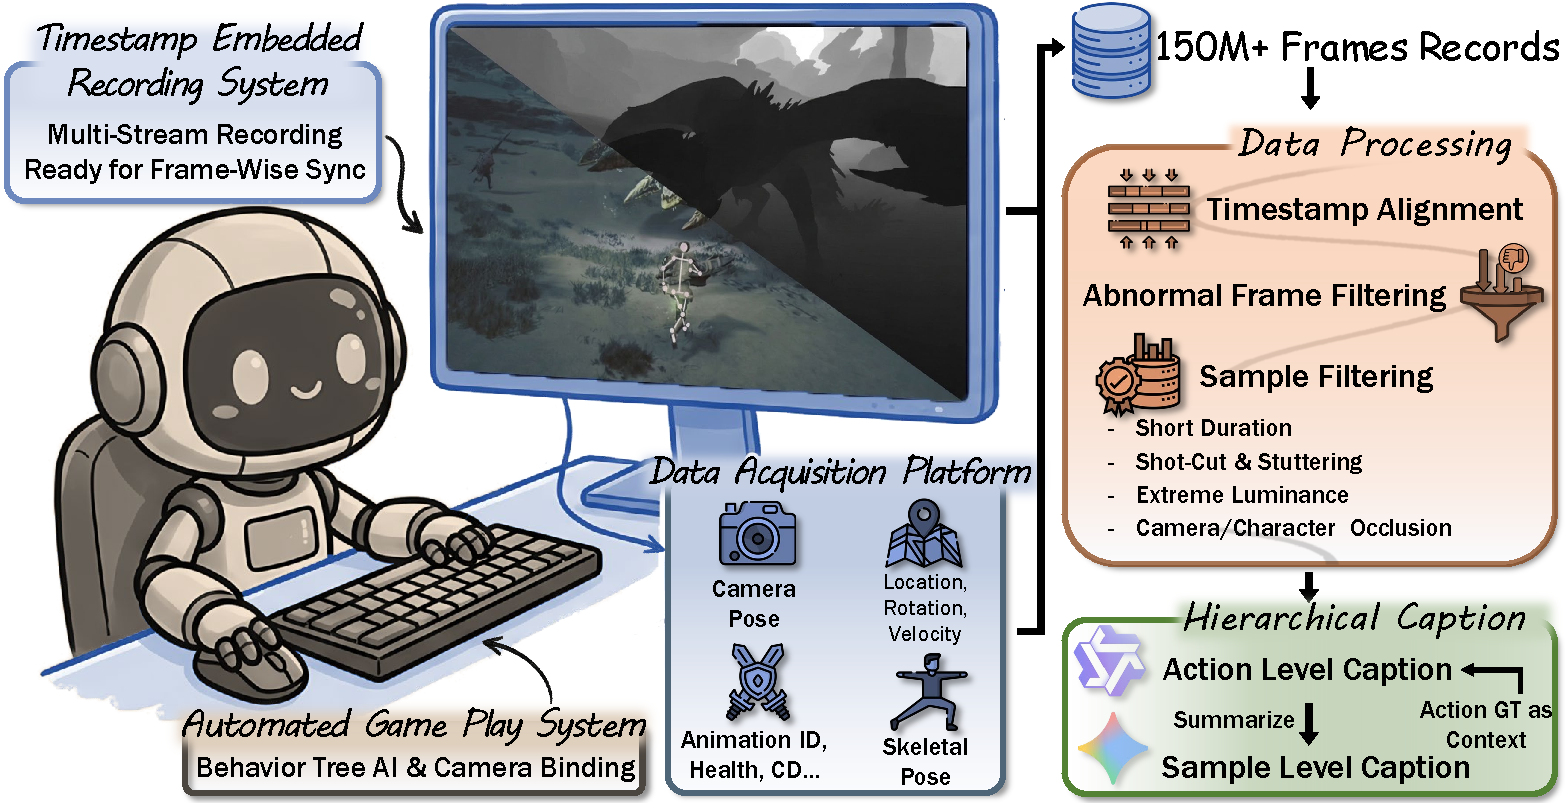
\includegraphics[width=0.9\linewidth]{figures/framework-arxiv.pdf}
\caption{The WildWorld dataset curation pipeline.}
\label{fig:framework}
\end{figure*}

\subsection{Data Acquisition Platform}

In the data acquisition stage, we collect the interaction data required for training and evaluating interactive world models, organized into three categories: actions, states, and observations.         
Actions specify the control inputs that drive interactions, states describe the underlying evolution of the game world, and observations correspond to its visual manifestations.
These three types of data can be recorded at different stages of modern game execution.
In \textit{Monster Hunter: Wilds}, the game engine processes player inputs, maintains and updates the world state. 
While the rendering pipeline consumes information from the game engine to produce the final imagery.
Following this separation, we develop a dedicated game data acquisition platform engineered for the high fidelity record of various categories of data.

Specifically, we build our data acquisition platform to record both player actions and world states ground truth,
including the executed actions, absolute location, rotation, and velocities of the player character and monsters in the game world, their current animation IDs, and gameplay attributes such as health, stamina/mana-like resources as actions and states.
We additionally record the skeletal poses of both the player character and monsters.
For world observations, we instrument the rendering pipeline to record RGB frames, depth maps, and the intrinsic and extrinsic parameters of the in-game camera. We further remove the HUD by disabling the corresponding late stage shaders.
This yields clean, HUD free frames that better reflect the game world for training and evaluating interactive world models.

\subsection{Automated Game Record Pipeline}

Turning the captured raw streams into a usable and scalable dataset requires solving several challenges at the system level. 
On one hand, to enable long running collection with minimal human intervention, we implement automated gameplay system, including menu UI navigation and player action execution.
On the other hand, to recorded different interaction data captured by separate tools, we design a robust recording system with embedded timestamps, to facilitate subsequent cross source synchronization and alignment.

\noindent
\textbf{Automated Game Play System}.
\textit{Monster Hunter: Wilds} follows a quest-based structure in which each session tasks a party of up to four characters, one player-controlled protagonist and three NPC companions, with hunting one or two large monsters.
Our automation consists of two components.
For quest selection, we invoke the game engine's UI components to programmatically navigate in-game menus and randomly sample quest-NPC combinations, ensuring diverse coverage over maps, monsters, and team compositions.
For automated combat, we leverage the game's built-in rule-based companion AI.
We enable automated combat by leveraging the behavior trees that drive NPC companions to fight autonomously, and correspondingly adjust the in-game camera binding so that the entire party can act without human input.
A natural concern is whether rule-based AI yields overly repetitive behavior.
We argue that the resulting trajectories remain sufficiently diverse for two reasons.
First, the combinatorial action space is large: the AI must select among dozens of moves and continuously adjust timing and positioning in response to monster behavior, which itself is stochastic.
Second, the interaction between multiple AI-controlled characters and a reactive monster creates a high-dimensional dynamical system whose trajectories vary substantially across sessions, even under the same scripted logic.
During automated combat, the camera is managed by the game's native target-lock system, which dynamically adjusts the camera position and angle to keep the engaged monster within the field of view while maintaining visual stability.

\noindent
\textbf{Recording System}. We develop a recording system for the simultaneous recording of interaction data from multiple sources. 
For structured information represented in text form, such as actions and states, recording is straightforward.
At each engine tick, these interaction data are uniformly recorded, serialized in JSON format, and written to one local file.
Given that the full screen is typically occupied by the RGB frame in standard rendering setups, image frame such as RGB and depth require a different strategy for simultaneous record.
To achieve that, we develop a dedicated system based on OBS Studio and Reshade.
Specifically, a custom Reshade shader partitions the full display into four sub-windows, two of which present the RGB and depth frames from the rendering buffer.
In practice, we set the full display resolution to 2K, yielding sub-windows of 720p.
We further adapt a modified version of OBS Studio to simultaneously record different sub-windows of the screen as separate recording streams, allowing RGB and depth to be recorded with different encoding settings.
Specifically, RGB is recorded with lossy HEVC compression under variable bitrate control, using a target bitrate of 16 Mbps and a maximum of 20 Mbps, so as to reduce storage cost while maintaining high visual quality.
In contrast, depth is recorded losslessly to preserve geometric precision and avoid discontinuities caused by lossy compression.
In practice, we use the HEVC encoder with B frames enabled, and the resulting bitrate of the depth stream remains around 20 Mbps.
In addition, we embed timestamp information into the recordings of multiple sources, which serves as a unified basis to process them and obtain synchronized data samples in the next section. 

\subsection{Data Processing and Annotation Pipeline}

While the temporally tagged multi source recordings collected in the previous stage contain rich action, state, and observation data, they may still contain misalignment, duplicated or dropped frames caused by occasional runtime instability, and low quality or uninformative content such as occlusions and cutscenes, making them unsuitable for direct use by interactive world models.
We therefore apply a set of multi-dimensional filters to remove low-quality samples.
Based on the resulting samples, we further annotate hierarchical caption to support fine-grained modeling and evaluation.

\noindent
\textbf{Sample Filtering}.
We filter the samples along the following dimensions to improve the overall data quality.
\begin{itemize}
    \item \textbf{Duration Filtering}.
    Very short samples provide limited value for interactive world modeling. 
    We therefore discard samples shorter than 81 frames.
    
    \item \textbf{Temporal Continuity Filtering}.
    Given the state record in every frame of samples is associated with a timestamp, we can directly measure the temporal gap between adjacent frames. 
    Excessive gaps typically indicate either stuttering in the game or recording system, or transitions into non-combat content such as cutscenes. 
    The latter can be identified in our data, since our platform only records data during combat or travel.
    We discard any sample in which the gap between two adjacent frames exceeds 1.5 times the target frame interval, \textit{i.e.}, approximately 50\,ms at 30 FPS.

    \item \textbf{Luminance Filtering}.
    Overly bright or dark visuals in games can create visually distinctive gameplay experiences, for example in combat effects or in nighttime scenes.
    However, such samples are less suitable for stable model training.
    We apply a simple filter based on the luma channel in YUV color space of the RGB frames, and remove samples with more than 15 consecutive frames of extremely high or low average brightness.

    \item \textbf{Camera Occlusion Filtering}.
    We remove samples with foreground occlusion, such as rocks, trees, or other scene geometry blocking the character. 
    We detect such cases using the spring-arm behavior of the third-person camera: when occlusion occurs, the arm contracts, leading to an abnormally small camera–character distance; 
    therefore, we discard samples whose recorded distances fall below a threshold for a sustained number of frames.
    We further exclude samples with abrupt player position changes, such as fast travel, as they break visual continuity.

    \item \textbf{Character Occlusion Filtering}.
    Severe character overlap in the first frame cam introduce ambiguity into image to video generation.
    We identify inter character overlap by projecting 3D skeletal keypoints onto screen coordinates in the first frame and discarding samples in which the overlap area between characters exceeds 30\% of either character's projected area.
\end{itemize}

\noindent
\textbf{Hierarchical Caption Annotations}
Fine-grained captions are important for capturing interaction details and enabling the training of more precisely controllable models, for example through prompt switching~\cite{ji2025memflow,yang2025longlive}.
Leveraging the action annotations provided in WildWorld, we segment each sample into action sequences according to the frame wise action IDs, such that the action remains unchanged within each sequence, \textit{e.g.}, walking forward or charging a heavy attack.
For each sequence, we sample RGB frames at 1 FPS, resize them to 480p, and use Qwen3-VL-235B-A22B-Instruct served with vLLM to generate detailed captions.
To compensate for the model’s limited familiarity with game specific scenarios, we additionally include the corresponding action and state ground-truth in the prompt context.
We further provide sample level captions by summarizing all action sequence captions in one sample with Gemini 3 Flash.

\subsection{Dataset Statistics}

After processing and filtering, we yield WildWorld with 108 million frames and 119 annotation columns per frame.

\begin{figure*}[t]
\centering
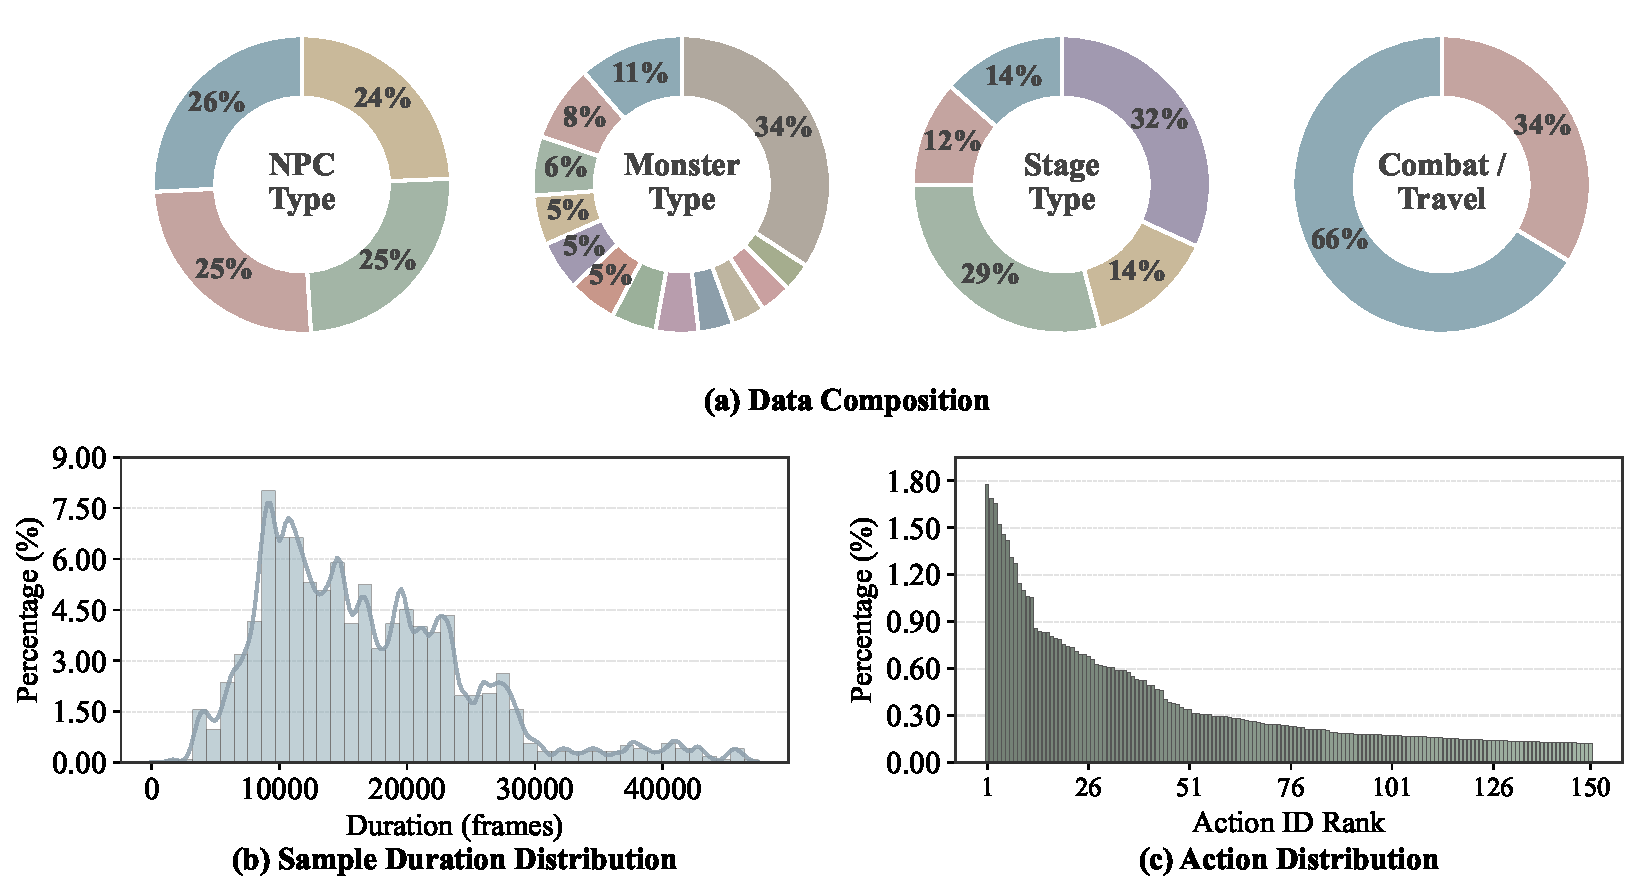
\includegraphics[width=\linewidth]{figures/dataset_overview_figure.pdf}
\caption{Wildworld dataset statistics overview. (a)~Data composition by character type, monster species, stage, and combat / travel ratio. (b)~Distribution of sample durations in frames. (c)~Frequency distribution of the top-150 action IDs, exhibiting a long-tail pattern.}
\label{fig:diversity_stats}
\end{figure*}

\noindent
\textbf{Entity Diversity}.
The dataset covers 29 unique monster species, 4 player characters, and 4 weapon types (Great Sword, Long Sword, Bow, Dual Blades).
As shown in \cref{fig:diversity_stats}\,(a), character types and weapon types are near-uniformly distributed, while monster species follow a long-tailed distribution dominated by a few frequent targets.
Multi-monster encounters also appear, with 7 secondary species present in the data.
This diversity is significant for training world models that generalize across entities and interaction patterns.

\noindent
\textbf{Scene Complexity}.
Gameplay spans 5 distinct stages set in an open-world map with diverse environments including deserts, snowy mountains, forests, swamps, and wastelands, under varying weather (sunny, rainy) and time-of-day (day, night) conditions.
As shown in \cref{fig:diversity_stats}\,(a), approximately 66\% of clips capture active combat, while the remaining 34\% depict traversal on mounts, providing a broad range of interaction contexts for training and evaluating world models.

\noindent
\textbf{Temporal and Spatial Dynamics}.
\cref{fig:diversity_stats}\,(b) shows the distribution of sample durations.
The majority of clips span 4,000 to 28,000 frames, while a smaller subset exceeds 40,000 frames (over 30 minutes of gameplay), capturing extended combat sequences or exploration that demand long-horizon consistency.
Spatially, the camera-to-character distance has a median of 15.69 units and the character-to-monster distance a median of 12.63 units. These close proximities ensure that the character and monster are prominently featured in the video frames, with clear visibility of their actions and state changes.

\noindent
\textbf{Action Richness}.
Each frame's character state is encoded as a (weapon type, bank ID, motion ID) triplet, yielding 5,960 unique character action triplets across 24 banks and 455 motion IDs.
These actions span movement, attacks, evasion, defense, item usage, and inter-action transitions, covering the full range of in-game interactions.
Monsters exhibit 2,132 unique action pairs across 13 banks and 527 motion IDs.
\cref{fig:diversity_stats}\,(c) shows the frequency of the top-150 character action IDs, which account for 58.49\% of all samples and follow a long-tail distribution, indicating rich behavioral variety.

\section{WildBench Benchmark}

Evaluating interactive world models requires measuring not only visual plausibility, but also how well the model follows input actions and produces aligned states.
Leveraging the action and state ground-truth provided by WildWorld, we evaluate generated videos from four perspectives: video quality, camera control, action following, and state alignment.
Among these, action following and state alignment more directly evaluate how well a model follows input actions and responds with aligned states under interaction, both of which are central to interactive world modeling.
This distinguishes our benchmark from existing ones~\cite{li2025worldmodelbench,duan2025worldscore,ye2026mind}, which mainly emphasize perceptual quality, controllability, or physics plausibility.

\subsection{Evaluation Metric}

We comprehensively evaluate interactive world models from four perspectives: 

\noindent
\textbf{Video Quality} characterizes the overall perceptual quality of generated videos in terms of both motion and appearance. 
We evaluate this dimension using four VBench metrics~\cite{huang2024vbench}: Motion Smoothness (MS) assesses the smoothness and physical plausibility of generated motion; Dynamic Degree (DD) measures the magnitude of motion to penalize overly static videos; Aesthetic Quality (AQ) reflects the perceived artistic and visual appeal of the generated content; Image Quality (IQ) evaluates low-level visual distortions, such as over-exposure, noise, and blur.

\noindent
\textbf{Camera Control} is essential for interactive world models, as inaccurate viewpoint control can prevent the intended observations from being properly presented.
We quantitatively evaluate camera control by measuring the discrepancy between the ground-truth camera trajectories and the camera trajectories estimated from generated videos using a structure from motion model following CameraCtrl~\cite{he2024cameractrl}.
To reduce the impact of scale mismatch between trajectories from the game engine and those estimated from video, we apply a scalar alignment factor to the estimated translations before evaluation.
We then compute Absolute Trajectory Error (ATE) and Relative Pose Error (RPE) for both translation and rotation~\cite{sturm2012benchmark}.
ATE measures the absolute deviation from the ground-truth trajectory, reflecting the overall accuracy of camera control, while RPE measures the discrepancy between relative motions and is therefore more sensitive to local consistency and accumulated drift along the trajectory.
In practice, we estimate camera trajectories using ViPE~\cite{huang2025vipe}.

\noindent
\textbf{Action Following} evaluates whether the model responds to input actions with the corresponding behaviors in generated videos.
Since each sample may contain multiple actions, we perform evaluation at the action sequence level for finer-grained assessment.
Based on the frame-wise action ID annotations in WildWorld, we divide each sample into action segments within which the action remains unchanged.
For each segment, we extract the corresponding frame range from both the generated video and the ground-truth video, and use Gemini 3 Flash to judge whether they express the same action.
We further group actions into three categories, namely movement, fast displacement, and attack, based on their action IDs, and design detailed prompts for each category.
Each segment is assigned a score of 1 if the generated and ground-truth clips are judged to be consistent, and 0 otherwise.
The final score is the average over all segments.

\noindent
\textbf{State Alignment}.
We use the poses of the player character and monsters as a proxy for state, since pose directly reflects many underlying world states and can also indirectly reveal others, such as the death pose when health reaches zero.
Using the ground-truth skeletons in WildWorld, we extract key skeletal points and project them onto screen coordinates to obtain 2D trajectories for each sample.
For generated videos, we focus on settings based on image-to-video generation, where the first frame is the ground-truth.
Thus, we initialize keypoints from the first frame and track them in generated videos with TAPNext~\cite{zholus2025tapnext}. 
Then, we define the State Alignment score as the mean coordinate accuracy between the predicted and ground-truth trajectories over all keypoints.
For each keypoint, the coordinate accuracy is computed as the average fraction of frames whose predicted locations fall within thresholds of 4, 8, 16, and 32 pixels from the ground truth.
We note that while state evolution may be stochastic due to factors such as random events, alignment with the ground truth remains statistically meaningful over a number of samples.

\subsection{Data Curation}

It is worth noting that all samples in WildWorld dataset are, in principle, available for evaluation, allowing users to flexibly construct custom test sets based on scenario, difficulty, and other factors.
In this paper, we manually curate a representative set of 200 samples covering diverse difficulty levels, combat scenarios, character and monster types, and events such as skill usage, knockdowns, deaths, and critical hits.
Among them, 100 samples involve cooperation between the player and NPCs against monsters, while the other 100 consist of one on one combat between the player and a monster.
